
\documentclass[tikz, border=1mm]{standalone}

\usepackage{amsmath}

\usetikzlibrary{calc,angles,quotes}

\usepackage{tkz-euclide}

\begin{document}
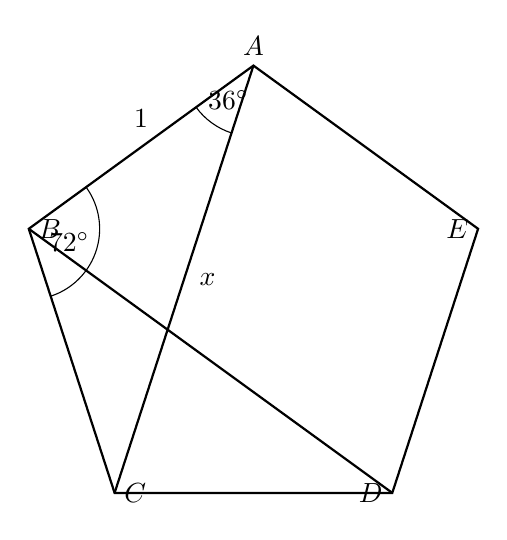
\begin{tikzpicture}[scale=3]

	% vertices of regular pentagon
	\foreach \i in {0,...,4}
	\coordinate (P\i) at ({90+72*\i}:1);

	% draw pentagon
	\draw[thick] (P0)--(P1)--(P2)--(P3)--(P4)--cycle;

	% draw diagonals
	\draw[thick] (P0)--(P2);
	\draw[thick] (P1)--(P3);

	% labels
	\node[above] at (P0) {$A$};
	\node[right] at (P1) {$B$};
	\node[right] at (P2) {$C$};
	\node[left]  at (P3) {$D$};
	\node[left]  at (P4) {$E$};

	% length labels
	\node at ($(P0)!0.5!(P1)+(0,0.12)$) {$1$};
	\node at ($(P0)!0.5!(P2)+(0.1,0)$) {$x$};

	% angle markers
	\pic[draw, "$36^\circ$", angle radius=0.9cm]
	{angle=P1--P0--P2};
	\pic[draw, "$72^\circ$", angle radius=0.9cm]
	{angle=P2--P1--P0};

\end{tikzpicture}
\end{document}
